%%%%%%%%%%%%%%%%%%%%%%%%%%%%%%%%%%%%%%%%%%%%%%%%%%%%%%%%%%%%%%%%%%%%%%%%%%
%                                                                        %
%      This file is part of the 'lilyglyphs' LaTeX package.              %
%                                ==========                              %
%                                                                        %
%              https://github.com/uliska/lilyglyphs                      %
%                                                                        %
%  Copyright 2012 by Urs Liska, git@ursliska.de                          %
%                                                                        %
%  'lilyglyphs' is free software: you can redistribute it and/or modify  %
%  it under the terms of the GNU General Public License as published by  %
%  the Free Software Foundation, either version 3 of the License, or     %
%  (at your option) any later version.                                   %
%                                                                        %
%  This program is distributed in the hope that it will be useful,       %
%  but WITHOUT ANY WARRANTY; without even the implied warranty of        %
%  MERCHANTABILITY or FITNESS FOR A PARTICULAR PURPOSE. See the          %
%  GNU General Public License for more details.                          %
%                                                                        %
%  You should have received a copy of the GNU General Public License     %
%  along with this program.  If not, see <http://www.gnu.org/licenses/>. %
%                                                                        %
%%%%%%%%%%%%%%%%%%%%%%%%%%%%%%%%%%%%%%%%%%%%%%%%%%%%%%%%%%%%%%%%%%%%%%%%%%

% This document is a playground for testing new commands before inserting them
% into the .sty file

\documentclass{scrartcl}

\usepackage{lilyglyphs}


%%%%%%%%%%%%%%%%%%%%%%%%
% Numbers and Dynamics %
%%%%%%%%%%%%%%%%%%%%%%%%

%\newcommand{\lilyNumber}[2][1.35]{\lilyText[#1]{#2}}


\begin{document}

%%%%%%%%%%%%%%%%%%%%%%%%
% Images               %
%%%%%%%%%%%%%%%%%%%%%%%%

\scriptsize
Try inverting glyphs: \crotchet*\crotchet[scale=-1,raise=2]


\newcommand{\lilyRFZtest}[1][]{%
    \mbox{%
        \lilyDynamics[#1]{r\hspace{0.035ex}fz}%
    }%
}

\lilyRFZ*. \lilyRFZ weiter

\section*{Rests}

This is normal text \lilyGlyph{rests.1o} \lilyDot around the dotted rest.

This is normal text\halfNoteRest TArount around the dotted rest.


This is normal text \halfNoteRestDotted* \lilyPrintMoreDots* a \lilyPrintMoreDots b 
TArount around the dotted rest.

This is a dotted half note rest:
\halfNoteRestDotted*[scale=0.5]|
\halfNoteRestDotted*[scale=1]|
\halfNoteRestDotted*[scale=1.5]|
\halfNoteRestDotted*[scale=2]|
\halfNoteRestDotted*[scale=3.5]|
\halfNoteRestDotted*[scale=5]|

Half note \halfNoteRest versus whole note \wholeNoteRestDotted*[scale=2].


This is a dotted crotchet rest: 
\crotchetRestDotted[scale=0.5] 
\crotchetRestDotted[scale=1]
\crotchetRestDotted[scale=1.5]
\crotchetRestDotted[scale=2]
\crotchetRestDotted[scale=3.5]
\crotchetRestDotted[scale=5]

this is a \crotchetRest in plain text and before a period \crotchetRest* !



Quaver rest \quaverRest with \semiquaverRest and without space \semiquaverRest*.\\
Dotted Quaver rest with \semiquaverRestDotted and without space \semiquaverRestDotted*.

\lilyGlyphByNumber{33} and space?

\lilyRFZ and space

\lilyDynamics{rfz} and space

\section*{Scripts}

This is a fermata \fermata* and text

\section*{Accidentals}
New \sharp accidental \sharpArrowdown and \sharpArrowdown*.\\
New \sharp accidental \sharpArrowup and \sharpArrowup*.\\
New \sharp accidental te \sharpArrowboth and \sharpArrowboth*.
New accidental \sharpSlashslashStem and \sharpSlashslashStem*,.\\
New accidental \sharpSlashslashslashStemstem and \sharpSlashslashslashStemstem*,.\\
New accidental \sharpSlashslashslashStem and \sharpSlashslashslashStem*,.\\
New accidental \sharpSlashslashStemstemstem and \sharpSlashslashStemstemstem*,.\\

\section*{Time Signatures}
	This is a normal Time signature: \lilyTimeSignature{3}{4}.
	
	As the plus sign is also directly accessible you can even
	write \lilyTimeSignature{3+7}{8+4} easily :-)
	
	One more option: \lilyTimeSignature{3}{8}\lilyText{+}\lilyTimeSignature{7}{4}. 
	
\section*{PGF/tikz}

Absatz, zusammen mit einem Notenkopf: 
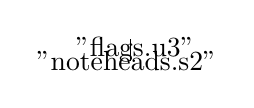
\begin{tikzpicture}
	\draw (0,0) node {\lilyGlyph{"noteheads.s2"}};
	\draw[semithick] (0.3ex,0) -- (0.3ex,0.8em);
	\draw (0.7ex,1ex) node {\lilyGlyph{"flags.u3"}};
\end{tikzpicture}

\Large
Neuer Absatz, zusammen mit einem Notenkopf: 
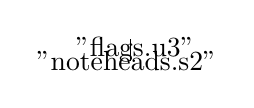
\begin{tikzpicture}
	\draw (0,0) node {\lilyGlyph{"noteheads.s2"}};
	\draw[semithick] (0.3ex,0) -- (0.3ex,0.8em);
	\draw (0.7ex,1ex) node {\lilyGlyph{"flags.u3"}};
\end{tikzpicture}

\normalsize
Neuer Absatz, zusammen mit einem Notenkopf: 
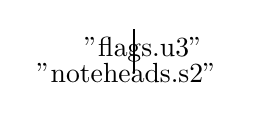
\begin{tikzpicture}[scale=2]
	\draw (0,0) node {\lilyGlyph{"noteheads.s2"}};
	\draw[semithick] (0.3ex,0) -- (0.3ex,0.8em);
	\draw (0.7ex,1ex) node {\lilyGlyph{"flags.u3"}};
\end{tikzpicture}

One sees: It is principally possible to combine graphical and textual elements with pgf/tikz,
but we definitely have to work on it some more: Especially it isn't scalable so far (explicitely or implicitely following text size)

	%\lilyNumber
	
\section*{PGF/tikz}

Absatz, zusammen mit einem Notenkopf: 
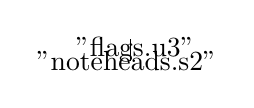
\begin{tikzpicture}
	\draw (0,0) node {\lilyGlyph{"noteheads.s2"}};
	\draw[semithick] (0.3ex,0) -- (0.3ex,0.8em);
	\draw (0.7ex,1ex) node {\lilyGlyph{"flags.u3"}};
\end{tikzpicture}

\Large
Neuer Absatz, zusammen mit einem Notenkopf: 
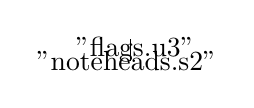
\begin{tikzpicture}
	\draw (0,0) node {\lilyGlyph{"noteheads.s2"}};
	\draw[semithick] (0.3ex,0) -- (0.3ex,0.8em);
	\draw (0.7ex,1ex) node {\lilyGlyph{"flags.u3"}};
\end{tikzpicture}

\normalsize
Neuer Absatz, zusammen mit einem Notenkopf: 
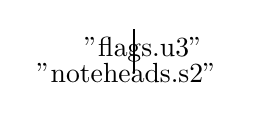
\begin{tikzpicture}[scale=2]
	\draw (0,0) node {\lilyGlyph{"noteheads.s2"}};
	\draw[semithick] (0.3ex,0) -- (0.3ex,0.8em);
	\draw (0.7ex,1ex) node {\lilyGlyph{"flags.u3"}};
\end{tikzpicture}

One sees: It is principally possible to combine graphical and textual elements with pgf/tikz,
but we definitely have to work on it some more: Especially it isn't scalable so far (explicitely or implicitely following text size)

\section*{exchange starred?}

If I write a \flat in a sentence, it is like I expect it.\\
And a \lilyRFZ is equally \lilyRF.

And a time signature \lilyTimeSignature{3}{4}?

A \lilyRFZ in text and at the end \lilyRFZ*.

General Dynamics \lilyDynamics{ff} aren't a problem \lilyDynamics{ff}.


	
>>>>>>> master
\end{document}